\documentclass[11pt]{ctexart}

\usepackage{multicol}
%\usepackage{mwe}
\usepackage{subfigure}
\usepackage{mathtools}
\usepackage{graphicx}
\usepackage{amsmath}
\usepackage{mathrsfs}
\usepackage[top=0.5in,bottom=1in,left=1in,right=1in]{geometry}
\usepackage{pdflscape}
\usepackage{times}
\usepackage{bm}
%\usepackage{setspace}
\usepackage{color}
\usepackage{caption}
\usepackage{amsmath}
\usepackage{amssymb}
\usepackage{CJK}
%\usepackage[final]{pdfpages}
\usepackage{listings}
\usepackage{textcomp}
\usepackage{xcolor}
\usepackage{algorithm2e}

\usepackage{algorithmicx}
\usepackage{algpseudocode}
\usepackage{hyperref}

\hypersetup{hidelinks,
	colorlinks=true,
	allcolors=black,
	pdfstartview=Fit,
	breaklinks=true}

\pagestyle{plain}




\begin{document}

\title{第二周实习报告20220309}
\author{宋欣源}
\date{\today}

\maketitle % need full-width title

\CTEXsetup[format={\Large\bfseries}]{section}

\section{第一,综述}

下面对于这五天实习的工作做一个报告。首先解决的问题是将batch_size变大1024.
我这周主要分成两个大的方向,CNN和RNN

\section{第一,CNN}
\subsection{综述}
在CNN领域,主要的思想是利用deepwise,普通CNN2d,和pointwise做特征提取。首先,我对各类CNN的基础性能

\subsection{实现}
模型0:普通CNN1d,三层
\begin{itemize}
  \item [1)]
  CNN1d(3,50,3*3)
  \item [2)]
  CNN1d(50,50,3*3)
  \item [3)]
  CNN1d(50,25,3*3)
  \item [4)]
  maxpool1d+dropout
  \item [5)]
  每个时间取最后
  \item [6)]
  两层全连接层,中间加relu

\end{itemize}
结果: batch\_size 1300, batchIC = 0.051,
pnl图(7epoch):
\begin{figure}[h!]
\begin{center}
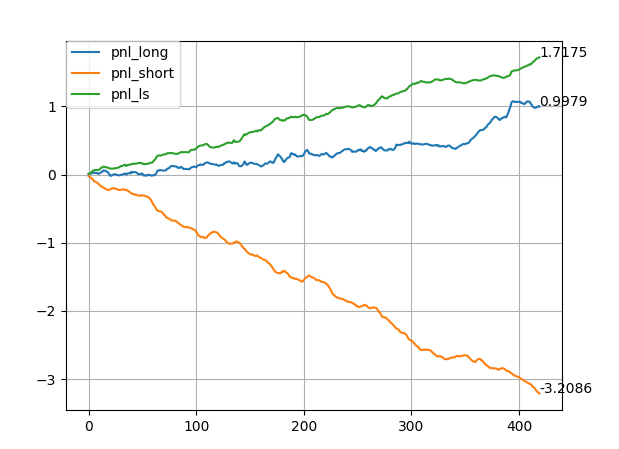
\includegraphics[width=0.5\textwidth]{2.PNG}
\end{center}
\caption{3layer CNN pnl figure}
\label{FIG.1}
\end{figure}

模型1:普通CNN2d
普通CNN2d要建立新的假象维度,把假象维度拆分成隐藏维度,假象维度只能是1,因为使用了假象维度,卷积核应该和特征数保持一致。(如果不一致,就要做下一层的CNN提取,目前先保持一致,采用卷积核大小为3)
\begin{itemize}
  \item [1)]
  CNN1d(1,50,3*3)
  \item [2)]
  maxpool1d+dropout
  \item [3)]
  每个时间取最后
  \item [4)]
  两层全连接层,中间加relu

\end{itemize}
结果: batch\_size 1300, batchIC = 0.041,
pnl图(7epoch):
\begin{figure}[h!]
\begin{center}
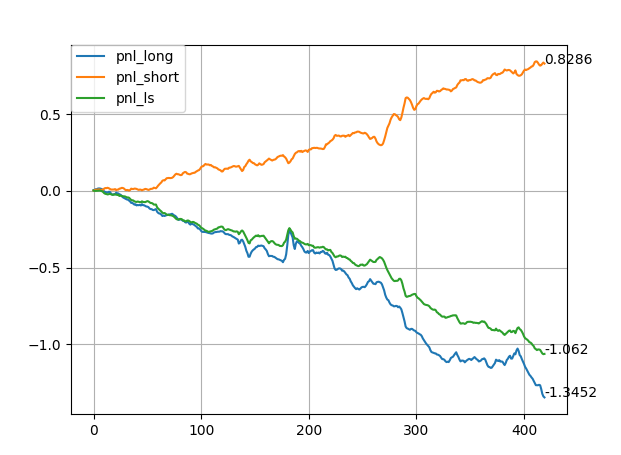
\includegraphics[width=0.5\textwidth]{1.PNG}
\end{center}
\caption{1layer CNN2d pnl figure}
\label{FIG.2}
\end{figure}

模型2:deepCNN2d
\begin{itemize}
  \item [1)]
  deepwise CNN2d(1300,1300,3*3, 1300)
  \item [2)]
  maxpool1d+dropout
  \item [3)]
  每个时间取最后和取时间平均都做尝试
  \item [4)]
  两层全连接层,中间加relu

\end{itemize}
结果: batch\_size 1300, batchIC = 0.047,
pnl图(7epoch):
\begin{figure}[h!]
\begin{center}
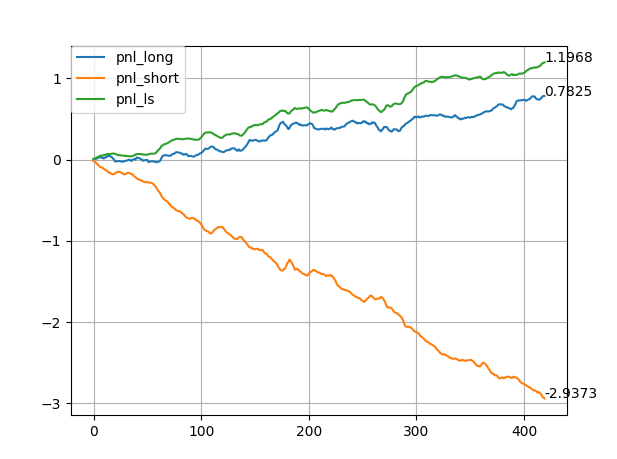
\includegraphics[width=0.5\textwidth]{4.PNG}
\end{center}
\caption{deep CNN2d pnl figure}
\label{FIG.3}
\end{figure}

模型3:pointCNN2d
\begin{itemize}
  \item [1)]
  deepwise CNN2d(1300,1300,3*3, 1300)
  \item [2)]
  maxpool1d+dropout
  \item [3)]
  pointwise CNN1d(T,1, 1)用cnn1d提取时间轴特征,时间轴提取到一
  \item [4)]
  两层全连接层,中间加relu

\end{itemize}
结果: batch\_size 1300, batchIC = 0.048,
pnl图(7epoch):
\begin{figure}[h!]
\begin{center}
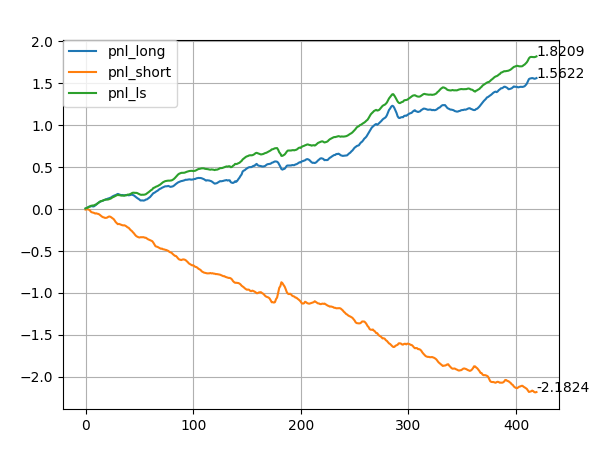
\includegraphics[width=0.5\textwidth]{5.PNG}
\end{center}
\caption{pointCNN2d pnl figure}
\label{FIG.4}
\end{figure}

模型4:deepCNN2d+pointCNN2d
\begin{itemize}
  \item [0)]
  deepwise CNN2d
  \item [1)]
  pointwise CNN2d
  \item [2)]
  maxpool1d+dropout
  \item [3)]
  pointwise CNN2d(T,1, 1*1)用cnn1d提取时间轴特征,时间轴提取到一
  \item [4)]
  两层全连接层,中间加relu

\end{itemize}
结果: batch\_size 1300, batchIC = 0.037,
pnl图(7epoch)
\begin{figure}[h!]
\begin{center}
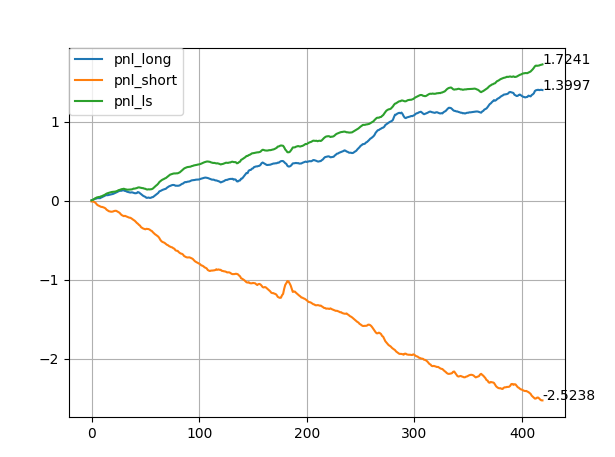
\includegraphics[width=0.5\textwidth]{3.PNG}
\end{center}
\caption{deepCNN+pointCNN pnl figure}
\label{FIG.5}
\end{figure}


模型5:deepCNN2d*2+pointCNN2d*2
每个卷积都用两层卷积来做,效果更好。
\begin{itemize}
  \item [0)]
  deepwise CNN2d
  \item [1)]
  pointwise CNN2d
  \item [2)]
  maxpool1d+dropout
  \item [3)]
  pointwise CNN2d(T,1, 1*1)用cnn1d提取时间轴特征,时间轴提取到一
  \item [4)]
  两层全连接层,中间加relu

\end{itemize}
结果: batch\_size 1300, batchIC = 0.047,


\subsection{改进思路}
非常多,我也不打算在参数维度和训练finetune上耽误时间,就单纯靠添加层和模块来提高质量。
\begin{itemize}
  \item [1)]
  从CNN的层数叠加,比如多层CNN2d(deepwise)叠加,因为deepwise不操作时间序列,所以基本上没有时间信息损失,可以反复叠加。
  \item [2)]
  时间轴上的特征提取,代替取时间最后一个数值或者取平均的办法。比如用pointwise提取时间轴特征,或者pointwise的分组。
  \item [3)]
  这些操作都是down操作,目的在于压缩维度。可以添加CNN进行扩展维度up,可以将压缩的维度重新扩展,再压缩,最后的曲线特征明显而且平滑。
  \item [4)]
  在模型上合理的使用maxpool,meanpool,minpool,batchnorm等
  \item [5)]
  全连接层深度增加,增加到5层左右

\end{itemize}

\section{其他思考}
还研究了elitwise和instancewise的两个思路,感觉用不上。

\section{总结}
我打算在CNN领域进行深度挖掘,把deeplab,bottleneck等CNN常用模型进行组合尝试,用自己的理解构造一些复杂CNN累积处理神经网络。这样过程更加有规律有轨迹可循,而不是随即和漫无目的地实现论文。

\begin{thebibliography}{1}
\bibitem{ref1} 华泰人工智能系列
\end{thebibliography}

\end{document} 